%%%%%%%%%%%%%%%%%%%%%%%%%%%%%%%%%%%%%%%%%%%%%%%%%%%%%%%%%%%%%%%%%%%%
%% I, the copyright holder of this work, release this work into the
%% public domain. This applies worldwide. In some countries this may
%% not be legally possible; if so: I grant anyone the right to use
%% this work for any purpose, without any conditions, unless such
%% conditions are required by law.
%%%%%%%%%%%%%%%%%%%%%%%%%%%%%%%%%%%%%%%%%%%%%%%%%%%%%%%%%%%%%%%%%%%%

% This theme was based on fibeamer theme 
% If you found any bugs please contact @karlosos
% This repository is hosted on github https://github.com/karlosos/zut-fibeamer/

\documentclass{beamer}
\usetheme[faculty=wi]{fibeamer}
\usepackage[utf8]{inputenc}
\usepackage[
  main=french,
  french
]{babel}

\title{Language C}
\subtitle{Université de Lorraine - Télécom Nancy}
\author{Omar CHIDA}

\usepackage{ragged2e}  % `\justifying` text
\usepackage{booktabs}  % Tables
\usepackage{tabularx}
\usepackage{tikz}      % Diagrams
\usetikzlibrary{calc, shapes, backgrounds}
\usepackage{amsmath, amssymb}
\usepackage{url}       % `\url`s
\usepackage{listings}  % Code listings
\frenchspacing
\begin{document}
  \frame[c]{\maketitle}

  \AtBeginSection[]{% Print an outline at the beginning of sections
    \begin{frame}<beamer>
      \frametitle{Chapitre \thesection}
      \tableofcontents[currentsection,currentsubsection,subsectionstyle=show/shaded/hide]
      \addtocounter{framenumber}{-1}
    \end{frame}}

  \begin{darkframes}
  	\section{Introduction}
  	\subsection{A propos de moi}
  	\begin{frame}{A propos de moi}
	  	\begin{columns}[T] % align columns
	  		\begin{column}{.71\textwidth}
	  			 \begin{itemize}
	  				\item Premier ligne de code à l'age de 14 ans.
	  				\item Hardline C++ Fanboy: 6 ans de C/C++.
	  				\item De nombreux projets dont un moteur de rendu, une application mobile entre autres codés en C/C++.
	  			\end{itemize}
	  		\end{column}%
	  		\hfill%
	  		\begin{column}{.25\textwidth}
	  			\begin{tikzpicture}[overlay,remember picture]
	  				\node[anchor=south east,xshift=-20pt,yshift=70pt]
	  				at (current page.south east) {
	  					
\includegraphics[width=35mm]{resources/omarito}
	  				};
	  			\end{tikzpicture}%
	  		\end{column}%
	  	\end{columns}
  	\end{frame}
  	\subsection{Organisation}
  	\begin{frame}{Organisation}
  		\framesubtitle{Comment ca va se passer?}%
  		\begin{itemize}
  			\item Cours, exercices, solutions et projets sertont sur \href{https://github.com/Darhal/TeachingC}{Github}.
  			\item Serveur \href{https://discord.gg/y9nYQ5A5Fz}{Discord} dédié pour les questions, aide et autre.
  			\item TD, TP et Projets seront en présentiel.
  			\item N'hésitez pas à m'interrompre à tout moment pour poser des questions.
  		\end{itemize}
  	\end{frame}
  	\subsection{L'objectif du Tutorat}
  	
  	\begin{frame}{L'objectif du Tutorat}
  		\begin{itemize}
	  		\item Vous familiariser avec la Langage C.
	  		\item Connaître les bonnes pratiques de programmation en C.
	  		\item Réussir les examens mais ça va aussi plus loin que ça.
	  		\item Compréhension approfondie des pointeurs et de la gestion de la mémoire en C.
	  		\item Bien comprendre l'outillage (Compilateur, Débogueur, autre).
  		\end{itemize}
    \end{frame}

	\begin{frame}{L'objectif du Tutorat}
		\framesubtitle{Ce que vous pourrez faire à la fin}%
		\begin{columns}[T] % align columns
			\begin{column}{.48\textwidth}
				\begin{tikzpicture}[overlay,remember picture]
					\node[anchor=south west,xshift=10pt,yshift=70pt]
					at (current page.south west) {
						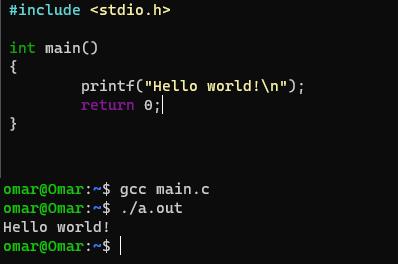
\includegraphics[scale=0.5]{resources/begin}
					};
				\end{tikzpicture}%
			\end{column}%
			%\hfill%
			\begin{column}{.065\textwidth}
			$\implies$
			\end{column}%
			\begin{column}{.48\textwidth}
				\begin{tikzpicture}[overlay,remember picture]
					\node[anchor=south east,xshift=-10pt,yshift=55pt]
					at (current page.south east) {
						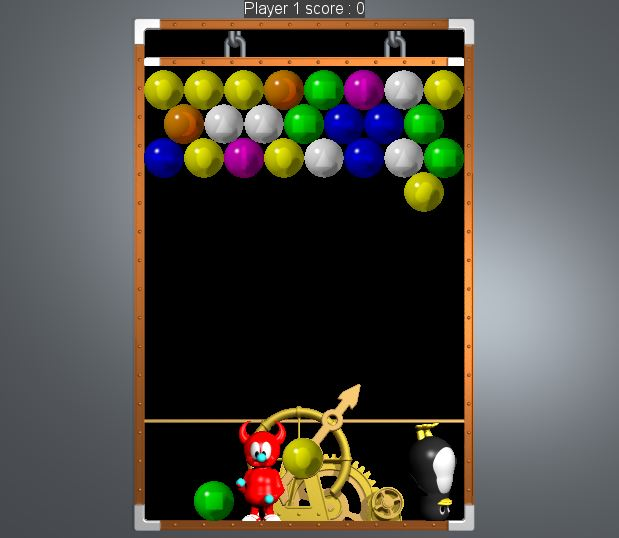
\includegraphics[scale=0.32]{resources/end}
					};
				\end{tikzpicture}%
			\end{column}%
		\end{columns}
	\end{frame}

  	\begin{frame}{L'objectif du Tutorat}
		\framesubtitle{Ce que nous allons faire ensemble}%
		\begin{itemize}
			\item Plein d'exercices (même style que les TD).
				\begin{itemize}
					\item Exercices liés aux structures de données.
					\item Savoir des techniques intelligentes pour avoir un code C plus rapide (de l'optimisation)
				\end{itemize}
			\item Il y aura un gros projet à la fin.
				\begin{itemize}
					\item Un jeu vidéo du style (Puzzle Bobble ou Mario).
					\item Jeu sur le terminal (style Snake).
					\item Émulateur de processeur ARM.
					\item Quelque chose de plus simple que ça? (n'hésitez pas à déposer vos idées).
				\end{itemize}
		\end{itemize}
	\end{frame}
	
  	\subsection{À propos de C}
  	\begin{frame}{À propos de C}
  		\framesubtitle{Un peu de connaissances générales}%
  		% dennis_ritchie
  		\begin{columns}[T] % align columns
  			\begin{column}{.76\textwidth}
  				 \begin{itemize}
  					\item Langage conçu par Dennis Ritchie et développé par lui et Bell labs.
  					\item Sortie en 1972 (Il y a 49 ans).
  					\item Utilisé dans le projet Unix développé par Dennis Ritchie et Ken Thompson entre autres.
  					\item A vu une évolution relativement petite.
  					\begin{itemize}
  						\item K\&R C, ANSI C, C99, C11, C17, C2x.
  					\end{itemize}
  					\item Aujourd'hui, C est considéré comme un langage de bas niveau.
  				\end{itemize}
  			\end{column}%
  			\hfill%
  			\begin{column}{.20\textwidth}
  				\begin{tikzpicture}[overlay,remember picture]
  					\node[anchor=south east,xshift=-10pt,yshift=50pt]
  					at (current page.south east) {
  						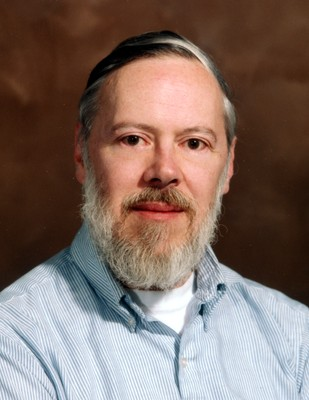
\includegraphics[width=30mm]{resources/dennis_ritchie}
  					};
  				\end{tikzpicture}%
  			\end{column}%
  		\end{columns}
  	\end{frame}
  
  	\subsection{Motivation: Pouquoi apprendre le C en 2021?}
  	\begin{frame}{Motivation: Pouquoi apprendre le C en 2021?}
  		\framesubtitle{C c'est cool !}%
  		\begin{itemize}
  			\item C est toujours pertinent et utile aujourd'hui pour beaucoup de choses.
  			\item Développement des noyaux (Kernel) et des systèmes d'exploitation
  			\item Systèmes embarqués (Véhicules, caméras, satellites, IoT, ...)
  			\item Développement de pilotes de périphériques (Device Drivers)
  			\item Bibliothèques et frameworks hautes performances (Numpy, ...)
  			\item Compilateurs et interprètes de nombreuses langues populaires (Java, Python, ...).
  			\item Moteurs de rendu et jeux vidéo.
  			\item Bref... partout où la performance est essentielle.
  		\end{itemize}
  	\end{frame}

	%%%%%%%%%% TODO %%%%%%%%%%%%%%%
  	\section{Compilation}
  	\begin{frame}{Compilation}
  		\framesubtitle{}%
  		\begin{itemize}
  			\item TODO !!!
  		\end{itemize}
  	\end{frame}
  
  	\subsection{Phase 1: Preprocessing}
  	\begin{frame}{Phase 1: Preprocessing}
  		\begin{block}{Preprocessing}
  			Le \alert{Preprocessing} (prétraitement) est la \alert{première} étape du pipeline de compilation. Au cours de laquelle:
  			\begin{itemize}
  				\item Les commentaires sont supprimés.
  				\item Les macros sont développées.
  				\item Les fichiers inclus sont développés.
  			\end{itemize}
  		\end{block}
  	  	\begin{exampleblock}{Exemple:}
  			Un \texttt{\#include <stdio.h>} sera remplacé à l'execution de la phase du preprocessing par le contenu du fichier \texttt{stdio.h}
  		\end{exampleblock}
  	\end{frame}
  	
  	\subsection{Phase 2: Compiling}
  	\begin{frame}{Phase 2: Compiling}
	  	\begin{block}{La Compilation}
	  		La \alert{Compilation} est la deuxième étape. Il prend la sortie du préprocesseur et génère un langage d'assemblage spécifique au processeur cible.
	  	\end{block}
		\begin{exampleblock}{Exemple:}
			- La commande "\texttt{gcc -S main.c}" arrête le pipeline de compilation avant l'étape d'assemblage.\\
			- Utilisez l'option "\texttt{-masm=intel}" pour obtenir l'assembleur en syntaxe Intel.
		\end{exampleblock}
  	\end{frame}
  
    \begin{frame}{Phase 2: Compiling}
  		\begin{columns}[T] % align columns
	  		\begin{column}{.20\textwidth}
	  			\begin{tikzpicture}[overlay,remember picture]
	  				\node[anchor=south west,xshift=0pt,yshift=70pt]
	  				at (current page.south west) {
	  					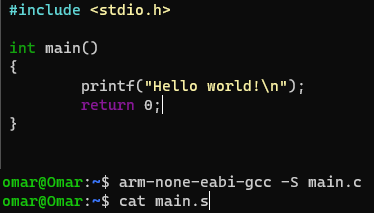
\includegraphics[scale=0.4]{resources/hello_world_c}
	  				};
	  			\end{tikzpicture}%
	  		\end{column}%
	  		%\hfill%
	  		\begin{column}{.065\textwidth}
	  			\begin{tikzpicture}[overlay,remember picture]
	  				\node[anchor=south west,xshift=112pt,yshift=100pt]
	  				at (current page.south west) {
	  					$\implies$
	  				};
	  			\end{tikzpicture}%
	  		\end{column}%
	  		\begin{column}{.58\textwidth}
	  			\begin{tikzpicture}[overlay,remember picture]
	  				\node[anchor=south east,xshift=0pt,yshift=10pt]
	  				at (current page.south east) {
	  					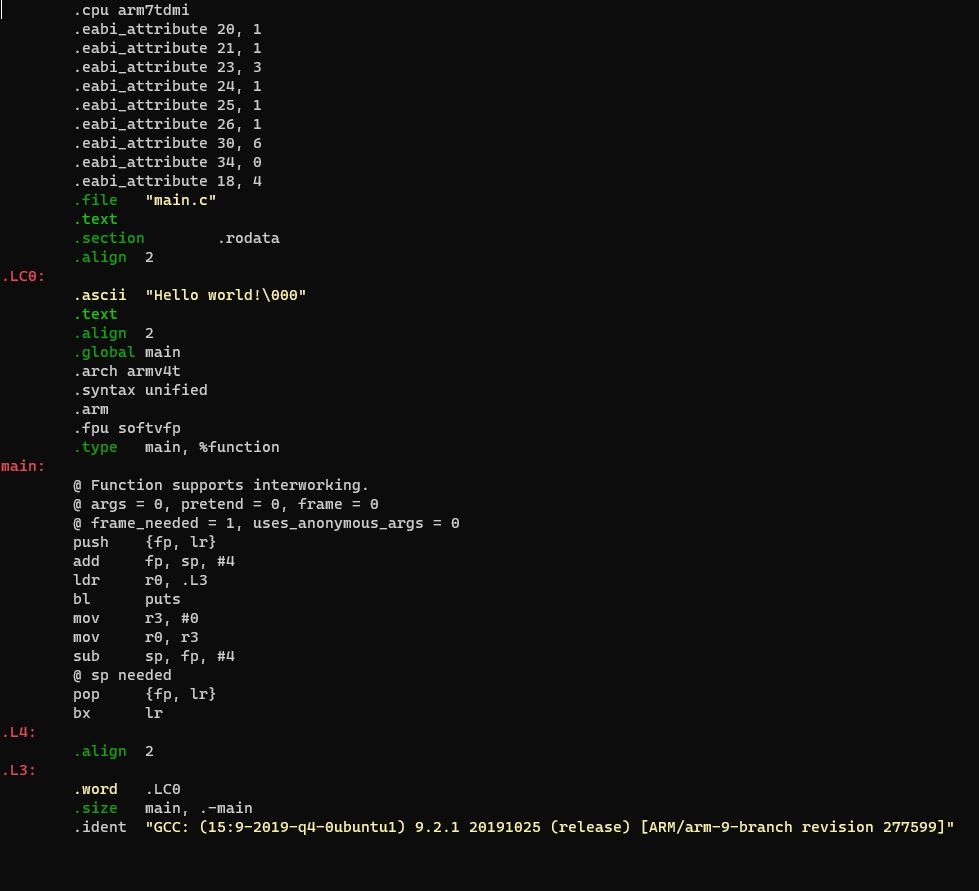
\includegraphics[scale=0.3]{resources/hello_world_arm}
	  				};
	  			\end{tikzpicture}%
	  		\end{column}%
	  	\end{columns}
  	\end{frame}
  	
  	\subsection{Phase 3: Assemblage}
  	\begin{frame}{Phase 3: Assemblage}
  		\begin{block}{L'Assemblage}
  			\alert{L'assemblage } est la troisième étape de la compilation. L'assembleur convertira le code d'assemblage en code binaire (code machine\footnote[frame]{Des zéros et uns}). Ce code est également appelé \alert{code objet}.
  		\end{block}
  		\begin{exampleblock}{Exemple:}
  			- La commande "\texttt{gcc -c main.c}" arrête le pipeline de compilation à l'étape de l'assemblage.\\
  		\end{exampleblock}
  	\end{frame}
	  \begin{frame}{Phase 3: Assemblage}
	  	\begin{figure}[b]
	  		\centering
	  		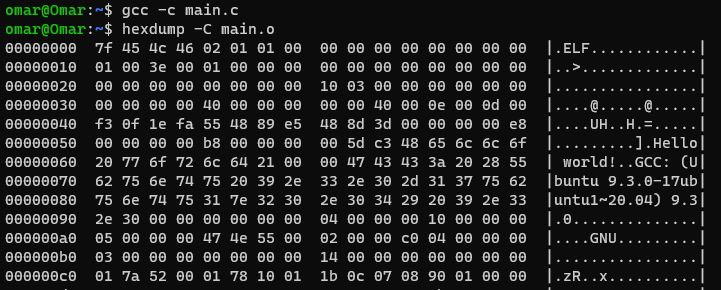
\includegraphics[scale=0.5]{resources/hello_world_o}
	  		\caption{Une representation hexadécimale du contenu du fichier binaire "main.o"}
	  	\end{figure}
	  \end{frame}
  	
	\subsection{Phase 4: Linking}
	\begin{frame}{Phase 4: Linking}
		\begin{block}{Édition du lien}
			\alert{L'édition du lien } est la dernière étape de la compilation. L'éditeur de liens \alert{fusionne } tout le code objet de plusieurs modules en un seul. \alert{Si} une fonction d'une bibliothèque est utilisée, l'éditeur de liens \alert{liera} le code actuel avec le code de la fonction utilisée \alert{fourni} par la bibliothèque.
		\end{block}
		\begin{alertblock}{N.B:}
			Il existe deux types de liaison:
			\begin{itemize}
				\item La \alert{liaison statique}.
				\item La \alert{liaison dynamique}.
			\end{itemize}
		\end{alertblock}
	\end{frame}

	\subsection{Phase 4: Linking}
	\begin{frame}{Phase 4: Linking}
		\begin{alertblock}{N.B:}
			Il existe deux types de liaison:
			\begin{itemize}
				\item Dans la \alert{liaison statique}, l'éditeur de liens fait une copie de toutes les fonctions de bibliothèque utilisées dans le fichier exécutable.
				\begin{itemize}
					\item Windows: l'extension `\texttt{.lib}'
					\item Linux \& MacOS: l'extension `\texttt{.a}'
				\end{itemize}
				\item En \alert{liaison dynamique}, le code n'est pas copié, il suffit juste d'ajouter la bibliothèque dans le même dossier que l'exécutable pour pouvoir exécuter le programme.
				\begin{itemize}
					\item Windows: l'extension `\texttt{.dll}'
					\item Linux: l'extension `\texttt{.so}'
					\item MacOS: l'extension `\texttt{.dylib}'
				\end{itemize}
			\end{itemize}
		\end{alertblock}
	\end{frame}
	  	
  	\section{La langage C}
  	\subsection{Les bases}
  	\begin{frame}{In the beginning there was main}
  		\begin{block}{La fonction main}
  			La fonction \alert{main} est le point d'entrée du programme \footnote[frame]{l'exécutable}.
  		\end{block}
  		\begin{exampleblock}{Profiles possibles:}
  			\begin{itemize}
  				\item \texttt{int main()}
  				\item \texttt{int main(int argc, char** argv)}
  			\end{itemize}
  		\end{exampleblock}
  		\begin{alertblock}{Profiles qui compile mais avec un Warning:}
  			\begin{itemize}
	  			\item \texttt{void main()}
	  			\item \texttt{void main(int argc, char** argv)}
  			\end{itemize}
  		\end{alertblock}
  	\end{frame}
  
  	\begin{frame}{In the beginning there was main}
		\framesubtitle{Les arguments de main}
		\begin{itemize}
			\item \alert{argc}: Indique le nombre d'arguments passés au programme. la valeur minimale de \texttt{argc} est 1 car le premier argument est toujours le nom du programme.
			\item \alert{argv}: Un tableau de chaîne contenant les arguments passés au programme, \texttt{argv[0]} est le nom du programme, \texttt{argv[1]} est le nom du premier argument, et ainsi de suite
		\end{itemize}
  	\end{frame}
  
  	\begin{frame}{In the beginning there was main}
	  	\begin{exampleblock}{Exemple:}
	  		Soit la commande suivante:~~"\texttt{./a.out abc w 23 1}" \\
	  		- \texttt{argc}: vaut 5 \\
	  		- \texttt{argv[0]}: est la chaine "./a.out" \\
	  		- \texttt{argv[1]}: est la chaine "abc" \\
	  		- \texttt{argv[2]}: est la chaine "w" \\
	  		- \texttt{argv[3]}: est la chaine "23" \\
	  		- \texttt{argv[4]}: est la chaine "1" \\
	  	\end{exampleblock}
  	\end{frame}
  
  
  	\defverbatim[colored]\ifsignle{
	\begin{lstlisting}[language=C,tabsize=2]
if (some_condition)
	statment; // Une seule instruction, cad un seul point-virgule	
  	\end{lstlisting}}
  
    \defverbatim[colored]\ifmulti{
   	\begin{lstlisting}[language=C,tabsize=2]
if (some_condition) {
	statment_1;
	statment_2;
	// ...
	statment_N;
}
    \end{lstlisting}}

\defverbatim[colored]\ifelsesignle{
\begin{lstlisting}[language=C,tabsize=2]
if (some_condition)
	statment; // Une seule instruction, cad un seul point-virgule	
[[else
	statment2; // un seul point-virgule	
]]
\end{lstlisting}}

\defverbatim[colored]\ifelsemulti{
\begin{lstlisting}[language=C,tabsize=2]
if (some_condition1) {
	statment_1;
	// ...
	statment_N;
} [[ else if (some_condition2) {
	statment_1;
	// ...
	statment_N;
// Possibilite d'ajouter plusieurs blocs else if 
} ]] [[ else {
	statment_1;
	// ...
	statment_N;
} ]]
\end{lstlisting}}
  	\begin{frame}{Les conditions}
  		\begin{block}{Syntax: Première possibilité}
  			\ifelsesignle
  		\end{block}
		\begin{alertblock}{N.B:}
			Ce qui est entre mis entre $\big[\big[~~...~~\big]\big]$ est facultatif
		\end{alertblock}
  	\end{frame}
  	
	\begin{frame}{Les conditions}
		  		\begin{block}{Syntax: Deuxième possibilité}
			\ifelsemulti
		\end{block}
	\end{frame}

\defverbatim[colored]\ifexampleone{
\begin{lstlisting}[language=C,tabsize=2]
int i = 0;
if (i--)
	puts("Hello World");
\end{lstlisting}}

\defverbatim[colored]\ifexampletwo{
\begin{lstlisting}[language=C,tabsize=2]
int i = -1;
if (i++)
	puts("Hello World");
\end{lstlisting}}

\defverbatim[colored]\ifexamplethree{
\begin{lstlisting}[language=C,tabsize=2]
int i = -1;
if (i++)
	if (++i)
		if ('c')
			puts("Hello World");
\end{lstlisting}}

	\begin{frame}{Les conditions}
		\begin{block}{Comment une condition est évaluée?}
			Le type \alert{booléen } n'existe pas en C. Si une expression est évaluée à 0, elle est considérée comme \alert{False}, sinon elle est considérée comme \alert{True}.
		\end{block}
	\end{frame}

	\begin{frame}{Les conditions: Exemple}	
		\begin{center}
			\begin{minipage}[t]{0.48\linewidth}
				\text{Example 1:}
				\ifexampleone
			\end{minipage}
			\qquad
			\begin{minipage}[t]{0.48\linewidth}
				\text{Example 2:}
				\ifexampletwo
			\end{minipage}
			\begin{minipage}[t]{0.48\linewidth}
				\text{Example 3:}
				\ifexamplethree
			\end{minipage}
		\end{center}
	\end{frame}

	\begin{frame}{Les conditions: Exemple}	
		\text{Example 1: \alert{(N'affiche rien)}}
		\ifexampleone
		\text{Example 2: \alert{(Affiche "Hello World")}}
		\ifexampletwo
		\text{Example 3: \alert{(Affiche "Hello World")}}
		\ifexamplethree
	\end{frame}

\defverbatim[colored]\forsyntax{
\begin{lstlisting}[language=C,tabsize=2]
for (initialisation; condition; increment) {
	// Une seule instruction, cad un seul point-virgule
}

\end{lstlisting}}
\defverbatim[colored]\forsyntaxtwo{
\begin{lstlisting}[language=C,tabsize=2]
for (initialisation; condition; increment)
	statment;
\end{lstlisting}}

\defverbatim[colored]\forWrittenUsingWhile{
\begin{lstlisting}[language=C,tabsize=2]
initialisation;
while (condition) {
	// ...
	increment;
}
\end{lstlisting}}


	\begin{frame}{Les boucles}	
		\begin{block}{Syntax: boucle pour}
			\forsyntax
			L'instruction \alert{d'initialisation } n'est exécutée qu'au début de la boucle. La \alert{condition} est vérifiée à chaque itération, \alert{l'instruction d'incrémentation} est également exécutée à chaque itération
		\end{block}
		\begin{alertblock}{Une boucle for peut être écrite comme une boucle while}
			\forWrittenUsingWhile
		\end{alertblock}
	\end{frame}

\defverbatim[colored]\forExmpOne{
\begin{lstlisting}[language=C,tabsize=2]
for (int i = 0; i < 10; i++)
	for (int j = 0; j < 20; j++)
		puts("Hello World");
\end{lstlisting}}

\defverbatim[colored]\forExmpTwo{
\begin{lstlisting}[language=C,tabsize=2]
for (;;)
	puts("Hello World");
\end{lstlisting}}

	\begin{frame}{Les boucles}
		\begin{block}{Syntax: boucle pour}
			Comme la syntaxe du \texttt{if}, la boucle pour peut être écrite de cette manière:
			\forsyntaxtwo
		\end{block}
		\begin{center}
			\begin{minipage}[t]{0.48\linewidth}
				\text{Example 1:}
				\forExmpOne
			\end{minipage}
			\begin{minipage}[t]{0.48\linewidth}
				\text{Example 2:}
				\forExmpTwo
			\end{minipage}
		\end{center}
	\end{frame}
	

\defverbatim[colored]\forExmpThree{
\begin{lstlisting}[language=C,tabsize=2]
for (int i = -1; i < 10; i++) {
	break;
	printf("Hello World\n");
}
\end{lstlisting}}

\defverbatim[colored]\forExmpFour{
\begin{lstlisting}[language=C,tabsize=2]
for (int i = -1; i < 10; i++) {
	if (i > 3) continue;
	printf("Hello World\n");
}
\end{lstlisting}}

\defverbatim[colored]\forExmpFive{
\begin{lstlisting}[language=C,tabsize=2]
for (int i = -1; i < 10; i++) {
	continue;
	printf("Hello World\n");
}
\end{lstlisting}}
	
	\begin{frame}{Les boucles}
		\begin{center}
			\begin{minipage}[t]{0.8\linewidth}
				Example 1: (\alert{Affiche 200 "Hello World"})
				\forExmpOne
			\end{minipage}
			\begin{minipage}[t]{0.8\linewidth}
				Example 2: (\alert{Affiche une infinité de "Hello World"})
				\forExmpTwo
			\end{minipage}
			\begin{minipage}[t]{0.8\linewidth}
				Example 3:
				\forExmpThree
			\end{minipage}
		\end{center}
	\end{frame}
	
	\begin{frame}{Les boucles}	
		\begin{minipage}[t]{0.8\linewidth}
			Example 3: (\alert{N'affiche rien})
			\forExmpThree
		\end{minipage}
		\begin{minipage}[t]{0.8\linewidth}
			Example 4:
			\forExmpFour
		\end{minipage}
		\begin{minipage}[t]{0.8\linewidth}
			Example 5:
			\forExmpFive
		\end{minipage}
	\end{frame}

	\begin{frame}{Les boucles}
		\begin{minipage}[t]{0.8\linewidth}
			Example 4:  (\alert{Affiche 5 "Hello World"})
			\forExmpFour
		\end{minipage}
		\begin{minipage}[t]{0.8\linewidth}
			Example 5: (\alert{N'affiche rien})
			\forExmpFive
		\end{minipage}
	\end{frame}

\defverbatim[colored]\doWhileSyntax{
\begin{lstlisting}[language=C,tabsize=2]
do {
	// ..
} while(condition);
\end{lstlisting}}
	\begin{frame}{Les boucles}
		\begin{block}{Syntax: boucle faire ... tantque}
			\doWhileSyntax
			La boucle continue de s'exécuter jusqu'à ce que la condition soit \alert{fausse}. 
			Il est similaire à une boucle tantque, sauf le fait qu'elle est garantie de s'exécuter au moins une fois.
		\end{block}
	\end{frame}
	
  	\subsection{Les structs}
  	\begin{frame}
  		
  	\end{frame}
  	
  	\subsection{Les enums}
  	\subsection{La mémoire}
  	\subsection{Les chaînes}
  	\subsection{Les pointeurs}
  	\subsection{Le keyword static}
  	
  	\section{Les outils}
  	\subsection{Compilateur: GCC/Clang}
  	\subsection{Débogueur: GDB}
  	\subsection{Valgrind}
  	
  	
  	
  	
  	
  	
  	
  	
  	
  	
  	
  	
  	
  	
  	
  	
  	
  	
  	
  	
  	
  	
  	
  	
  	
  	
  	
  	
  	
  	
  	
  	
  	
  	
  	
  	
 
    \section{Dark Frames}
    \subsection{Blind Text}
    \begin{frame}{Jabberwocky}
      \framesubtitle{Lewis Carroll}%
      \begin{tikzpicture}[overlay,remember picture]
        \node[anchor=south east,xshift=-30pt,yshift=35pt]
          at (current page.south east) {
            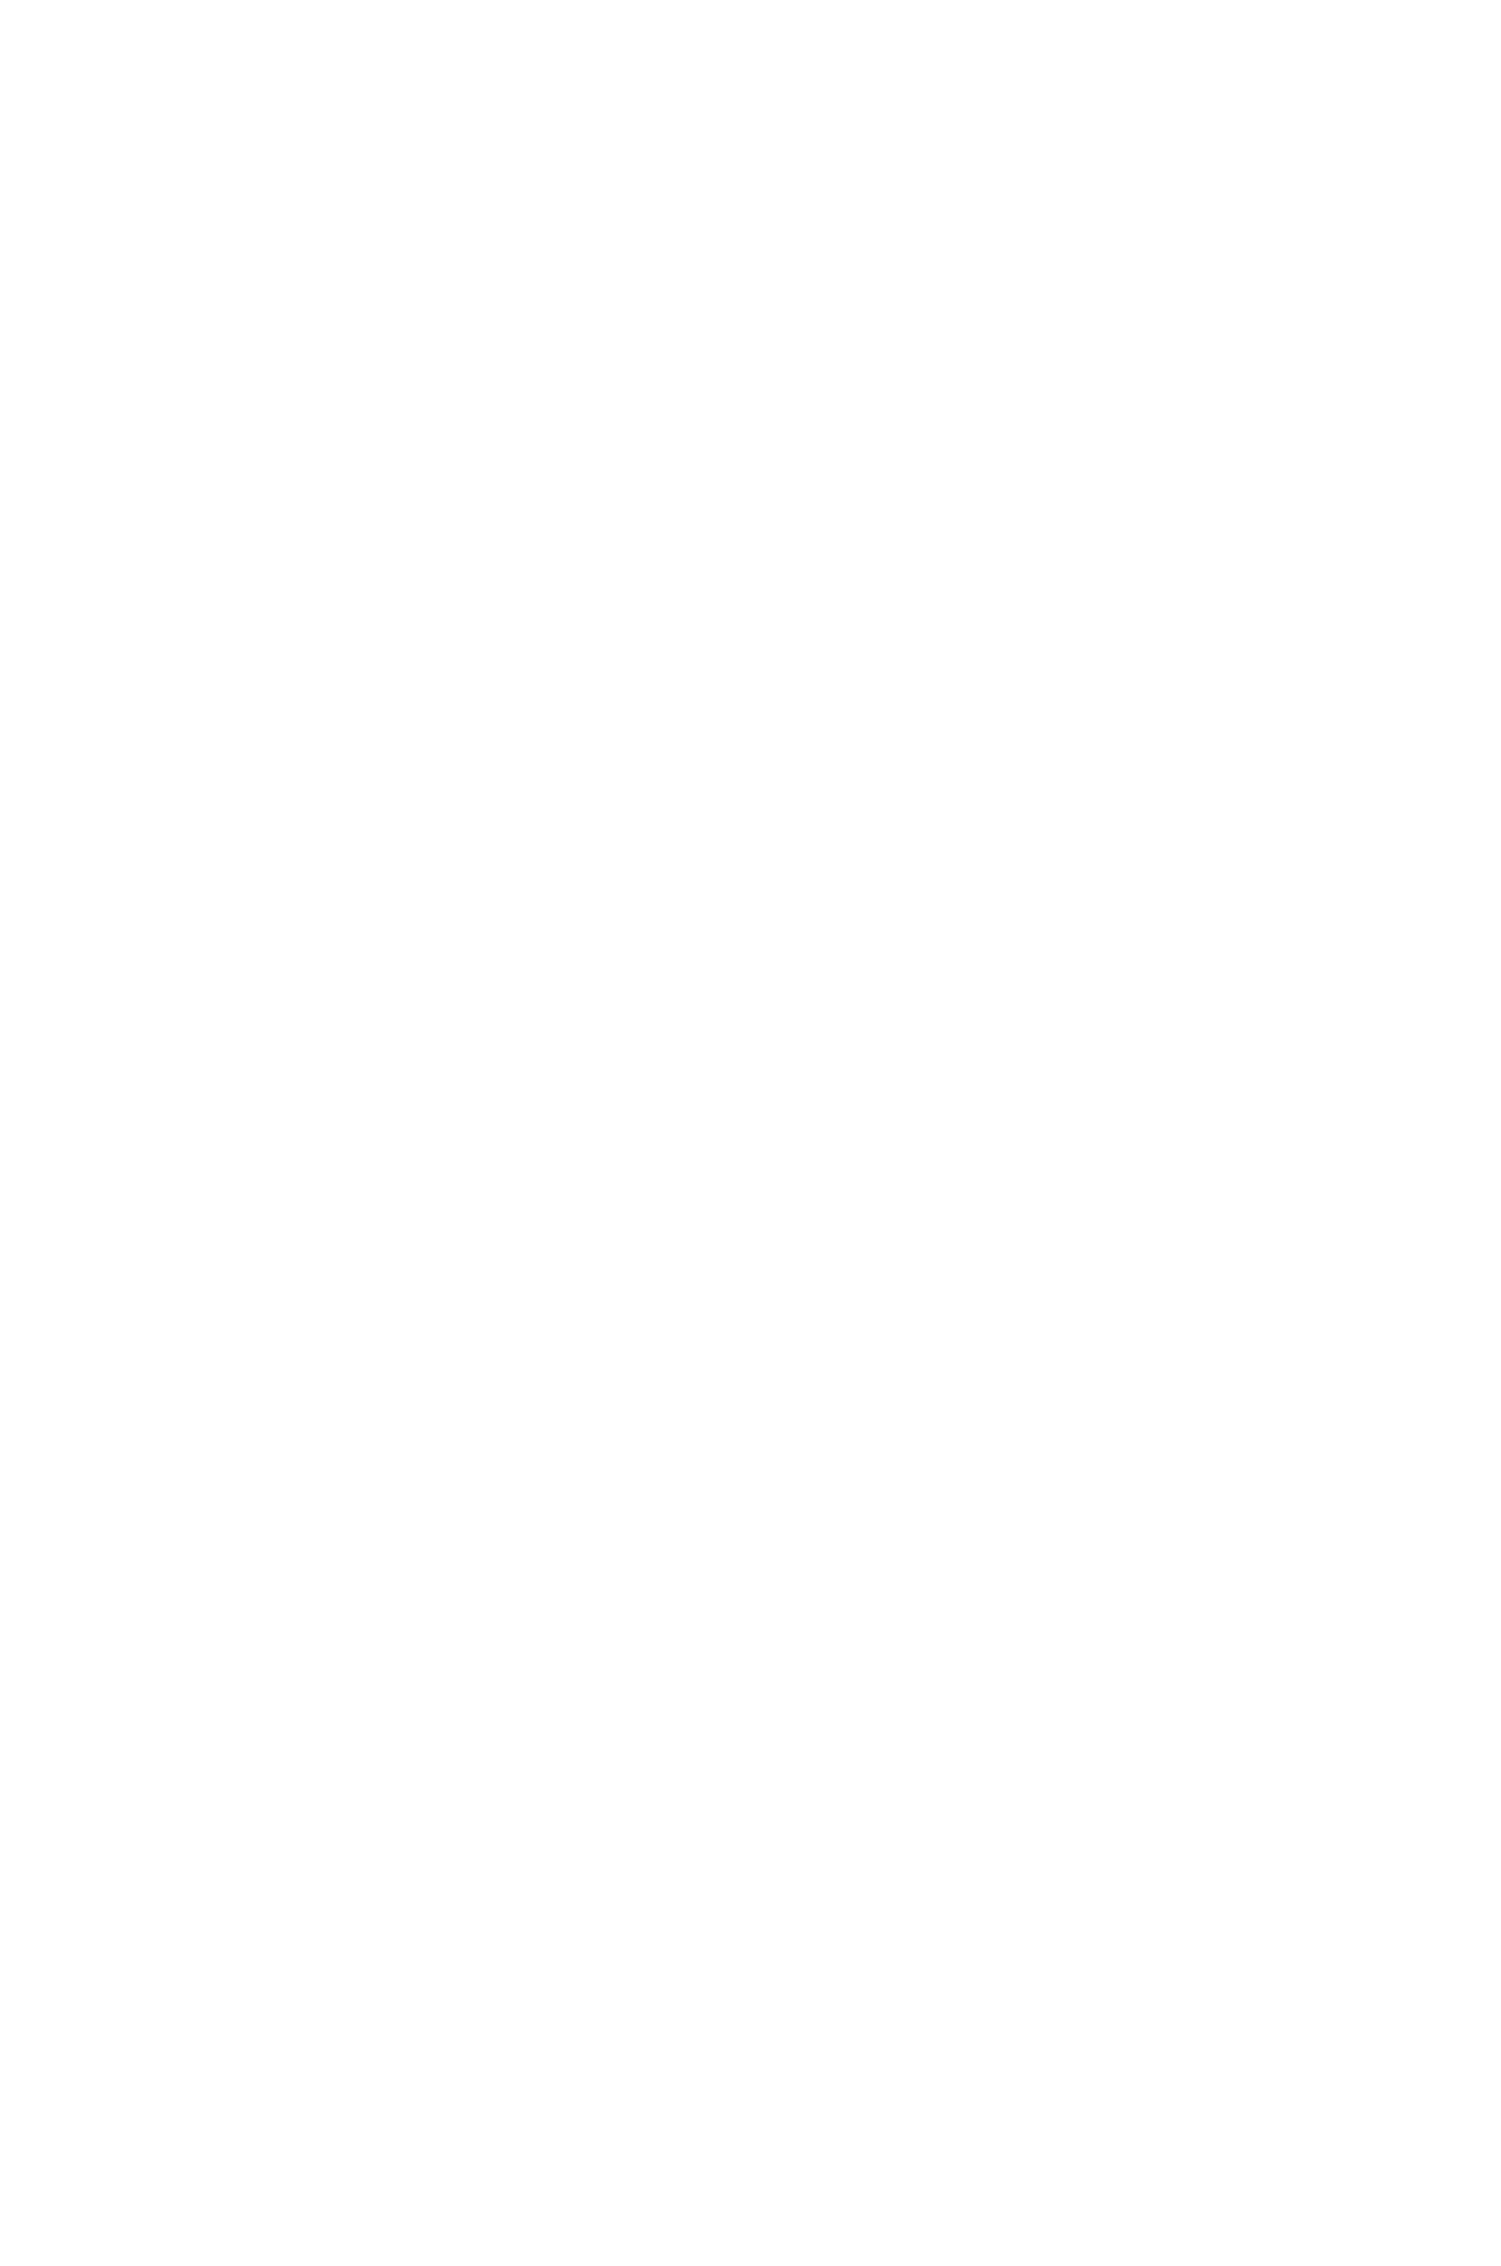
\includegraphics[width=35mm]{resources/jabberwocky-dark}
          };
      \end{tikzpicture}%
      'Twas brillig, and the slithy toves\\
      Did gyre and gimble in the wabe;\\
      All mimsy were the borogoves,\\
      And the mome raths outgrabe.\\\bigskip

      “Beware the Jabberwock, my son!\\
      The jaws that bite, the claws that catch!\\
      Beware the Jubjub bird, and shun\\
      The frumious Bandersnatch!”\\
    \end{frame}

    \begin{frame}[label=lists]{Lists and locales}
      \framesubtitle{Lorem ipsum dolor sit amet}
      \begin{columns}[onlytextwidth]
        \column{.5\textwidth}
          \begin{itemize}
            \item Nulla nec lacinia odio. Curabitur urna tellus.
            \begin{itemize}
              \item Fusce id sodales dolor. Sed id metus dui.
              \begin{itemize}
                \item Cupio virtus licet mi vel feugiat.
              \end{itemize}
            \end{itemize}
          \end{itemize}
        \column{.5\textwidth}
          \begin{enumerate}
            \item Donec porta, risus porttitor egestas scelerisque video.
            \begin{enumerate}
              \item Nunc non ante fringilla, manus potentis cario.
              \begin{enumerate}
                \item Pellentesque servus morbi tristique.
              \end{enumerate}
            \end{enumerate}
          \end{enumerate}
      \end{columns}
      \bigskip
      \justifying

      {\uselanguage{czech}Nechť již hříšné saxofony ďáblů
      rozzvučí síň úděsnými tóny waltzu, tanga a quickstepu!}
      {\uselanguage{slovak} Nezvyčajné kŕdle šťastných figliarskych
      ďatľov učia pri kótovanom ústí Váhu mĺkveho koňa Waldemara
      obžierať väč\-šie kusy exkluzívnej kôry.}
      {\uselanguage{english}The quick, brown fox jumps over a lazy
      dog. DJs flock by when MTV ax quiz prog. “Now fax quiz Jack!”}
    \end{frame}

    \subsection{Structuring Elements}
    \begin{frame}[label=simmonshall]{Text blocks}
      \framesubtitle{In plain, example, and \alert{alert} flavour}
      \alert{This text} is highlighted.

      \begin{block}{A plain block}
        This is a plain block containing some \alert{highlighted text}.
      \end{block}
      \begin{exampleblock}{An example block}
        This is an example block containing some \alert{highlighted text}.
      \end{exampleblock}
      \begin{alertblock}{An alert block}
        This is an alert block containing some \alert{highlighted text}.
      \end{alertblock}
    \end{frame}

    \begin{frame}[label=proof]{Definitions, theorems, and proofs}
      \framesubtitle{All integers divide zero}
      \begin{definition}
        $\forall a,b\in\mathds{Z}: a\mid b\iff\exists c\in\mathds{Z}:a\cdot c=b$
      \end{definition}
      \begin{theorem}
        $\forall a\in\mathds{Z}: a\mid 0$
      \end{theorem}
      \begin{proof}[Proof\nopunct]
        $\forall a\in\mathds{Z}: a\cdot 0=0$
      \end{proof}
    \end{frame}

    \subsection{Numerals and Mathematics}
    \begin{frame}[label=math]{Numerals and Mathematics}
      \framesubtitle{Formulae, equations, and expressions}
      \begin{columns}[onlytextwidth]
        \column{.20\textwidth}
          1234567890
        \column{.20\textwidth}
          \oldstylenums{1234567890}
        \column{.20\textwidth}
          $\hat{x}$, $\check{x}$, $\tilde{a}$,
          $\bar{a}$, $\dot{y}$, $\ddot{y}$
        \column{.40\textwidth}
          $\int \!\! \int f(x,y,z)\,\mathsf{d}x\mathsf{d}y\mathsf{d}z$
      \end{columns}
      \begin{columns}[onlytextwidth]
        \column{.5\textwidth}
          $$\frac{1}{\displaystyle 1+
            \frac{1}{\displaystyle 2+
            \frac{1}{\displaystyle 3+x}}} +
            \frac{1}{1+\frac{1}{2+\frac{1}{3+x}}}$$
        \column{.5\textwidth}
          $$F:\left| \begin{array}{ccc}
          F''_{xx} & F''_{xy} &  F'_x \\
          F''_{yx} & F''_{yy} &  F'_y \\
          F'_x     & F'_y     & 0
          \end{array}\right| = 0$$
      \end{columns}
      \begin{columns}[onlytextwidth]
        \column{.3\textwidth}
          $$\mathop{\int \!\!\! \int}_{\mathbf{x} \in \mathds{R}^2}
          \! \langle \mathbf{x},\mathbf{y}\rangle\,\mathsf{d}\mathbf{x}$$
        \column{.33\textwidth}
          $$\overline{\overline{a\alpha}^2+\underline{b\beta}
           +\overline{\overline{d\delta}}}$$
        \column{.37\textwidth}
          $\left] 0,1\right[ + \lceil x \rfloor - \langle x,y\rangle$
      \end{columns}
      \begin{columns}[onlytextwidth]
        \column{.4\textwidth}
          \begin{eqnarray*}
           e^x &\approx& 1+x+x^2/2! + \\
             && {}+x^3/3! + x^4/4!
          \end{eqnarray*}
        \column{.6\textwidth}
          $${n+1\choose k} = {n\choose k} + {n \choose k-1}$$
      \end{columns}
    \end{frame}

    \subsection{Figures and Code Listings}
    \begin{frame}[label=figs1]{Figures}
      \framesubtitle{Tables, graphs, and images}
      \begin{table}[!b]
        {\carlitoTLF % Use monospaced lining figures
        \begin{tabularx}{\textwidth}{Xrrr}
          \textbf{Faculty} & \textbf{With \TeX} & \textbf{Total} &
          \textbf{\%} \\
          \toprule
          Faculty of Informatics       & 1\,716  & 2\,904  &
          59.09 \\% 1433
          Faculty of Science           & 786     & 5\,275  &
          14.90 \\% 1431
          Faculty of $\genfrac{}{}{0pt}{}{\textsf{Economics and}}{%
          \textsf{Administration}}$    & 64      & 4\,591  &
          1.39  \\% 1456
          Faculty of Arts              & 69      & 10\,000 &
          0.69  \\% 1421
          Faculty of Medicine          & 8       & 2\,014  &
          0.40  \\% 1411
          Faculty of Law               & 15      & 4\,824  &
          0.31  \\% 1422
          Faculty of Education         & 19      & 8\,219  &
          0.23  \\% 1441
          Faculty of Social Studies    & 12      & 5\,599  &
          0.21  \\% 1423
          Faculty of Sports Studies    & 3       & 2\,062  &
          0.15  \\% 1451
          \bottomrule
        \end{tabularx}}
        \caption{The distribution of theses written using \TeX\ during 2010--15 at MU}
      \end{table}
    \end{frame}

    \begin{frame}[label=figs2]{Figures}
      \framesubtitle{Tables, graphs, and images}
      \begin{figure}[b]
        \centering
        % Flipping a coin
        % Author: cis
        \tikzset{
          head/.style = {fill = none, label = center:\textsf{H}},
          tail/.style = {fill = none, label = center:\textsf{T}}}
        \scalebox{0.65}{\begin{tikzpicture}[
            scale = 1.5, transform shape, thick,
            every node/.style = {draw, circle, minimum size = 10mm},
            grow = down,  % alignment of characters
            level 1/.style = {sibling distance=3cm},
            level 2/.style = {sibling distance=4cm},
            level 3/.style = {sibling distance=2cm},
            level distance = 1.25cm
          ]
          \node[shape = rectangle,
            minimum width = 6cm, font = \sffamily] {Coin flipping}
          child { node[shape = circle split, draw, line width = 1pt,
                  minimum size = 10mm, inner sep = 0mm, rotate = 30] (Start)
                  { \rotatebox{-30}{H} \nodepart{lower} \rotatebox{-30}{T}}
           child {   node [head] (A) {}
             child { node [head] (B) {}}
             child { node [tail] (C) {}}
           }
           child {   node [tail] (D) {}
             child { node [head] (E) {}}
             child { node [tail] (F) {}}
           }
          };

          % Filling the root (Start)
          \begin{scope}[on background layer, rotate=30]
            \fill[head] (Start.base) ([xshift = 0mm]Start.east) arc (0:180:5mm)
              -- cycle;
            \fill[tail] (Start.base) ([xshift = 0pt]Start.west) arc (180:360:5mm)
              -- cycle;
          \end{scope}

          % Labels
          \begin{scope}[nodes = {draw = none}]
            \path (Start) -- (A) node [near start, left]  {$0.5$};
            \path (A)     -- (B) node [near start, left]  {$0.5$};
            \path (A)     -- (C) node [near start, right] {$0.5$};
            \path (Start) -- (D) node [near start, right] {$0.5$};
            \path (D)     -- (E) node [near start, left]  {$0.5$};
            \path (D)     -- (F) node [near start, right] {$0.5$};
            \begin{scope}[nodes = {below = 11pt}]
              \node [name = X] at (B) {$0.25$};
              \node            at (C) {$0.25$};
              \node [name = Y] at (E) {$0.25$};
              \node            at (F) {$0.25$};
            \end{scope}
          \end{scope}
        \end{tikzpicture}}
        \caption{Tree of probabilities -- Flipping a coin\footnote[frame]{%
          A derivative of a diagram from \url{texample.net} by cis, CC BY 2.5 licensed}}
      \end{figure}
    \end{frame}

    \defverbatim[colored]\sleepSort{
      \begin{lstlisting}[language=C,tabsize=2]
  #include <stdio.h>
  #include <unistd.h>
  #include <sys/types.h>
  #include <sys/wait.h>

  // This is a comment
  int main(int argc, char **argv)
  {
          while (--c > 1 && !fork());
          sleep(c = atoi(v[c]));
          printf("%d\n", c);
          wait(0);
          return 0;
  }
    \end{lstlisting}}
    \begin{frame}{Code listings}{An example source code in C}
      \sleepSort
    \end{frame}

    \subsection{Citations and Bibliography}
    \begin{frame}[label=citations]{Citations}
      \framesubtitle{\TeX, \LaTeX, and Beamer}

      \justifying\TeX\ is a programming language for the typesetting
      of documents. It was created by Donald Erwin Knuth in the late
      1970s and it is documented in \emph{The \TeX
      book}~\cite{knuth84}.

      In the early 1980s, Leslie Lamport created the initial version
      of \LaTeX, a high-level language on top of \TeX, which is
      documented in \emph{\LaTeX : A Document Preparation
      System}~\cite{lamport94}. There exists a healthy ecosystem of
      packages that extend the base functionality of \LaTeX;
      \emph{The \LaTeX\ Companion}~\cite{MG94} acts as a guide
      through the ecosystem.

      In 2003, Till Tantau created the initial version of Beamer, a
      \LaTeX\ package for the creation of presentations. Beamer is
      documented in the \emph{User's Guide to the Beamer
      Class}~\cite{tantau04}.
    \end{frame}

    \begin{frame}[label=bibliography]{Bibliography}
      \framesubtitle{\TeX, \LaTeX, and Beamer}
      \begin{thebibliography}{9}
        \bibitem{knuth84}
            Donald~E.~Knuth.
            \emph{The \TeX book}.
            Addison-Wesley, 1984.
        \bibitem{lamport94}
            Leslie~Lamport.
            \emph{\LaTeX : A Document Preparation System}.
            Addison-Wesley, 1986.
        \bibitem{MG94}
            M.~Goossens, F.~Mittelbach, and A.~Samarin.
            \emph{The \LaTeX\ Companion}.
            Addison-Wesley, 1994.
        \bibitem{tantau04}
            Till~Tantau.
            \emph{User's Guide to the Beamer Class Version 3.01}.
            Available at \url{http://latex-beamer.sourceforge.net}.
        \bibitem{MS05}
            A.~Mertz and W.~Slough.
            Edited by B.~Beeton and K.~Berry.
            \emph{Beamer by example} In TUGboat,
              Vol. 26, No. 1., pp. 68-73.
      \end{thebibliography}
    \end{frame}

  \end{darkframes}
\end{document}
